\section{Neurobiology}\label{sec:neurobiology}
\qquad \todo{straightforward recap of the basics, more focus on topic-relevant details}
\subsection{Membrane Potential}\label{subsec:membrane-potential}
Nerve cells (neurons) have a resting membrane potential of roughly -70mV.
This electric potential is the result of a multitude of factors that ultimately decide the
different concentrations of ions inside and outside the cell, which in turn cause the potential difference.
The most important ions involved in this process are sodium ($Na^+$), potassium ($K^+$) and chloride ($Cl^-$).
\begin{wrapfigure}[21]{r}{0.5\textwidth}
		\centering
		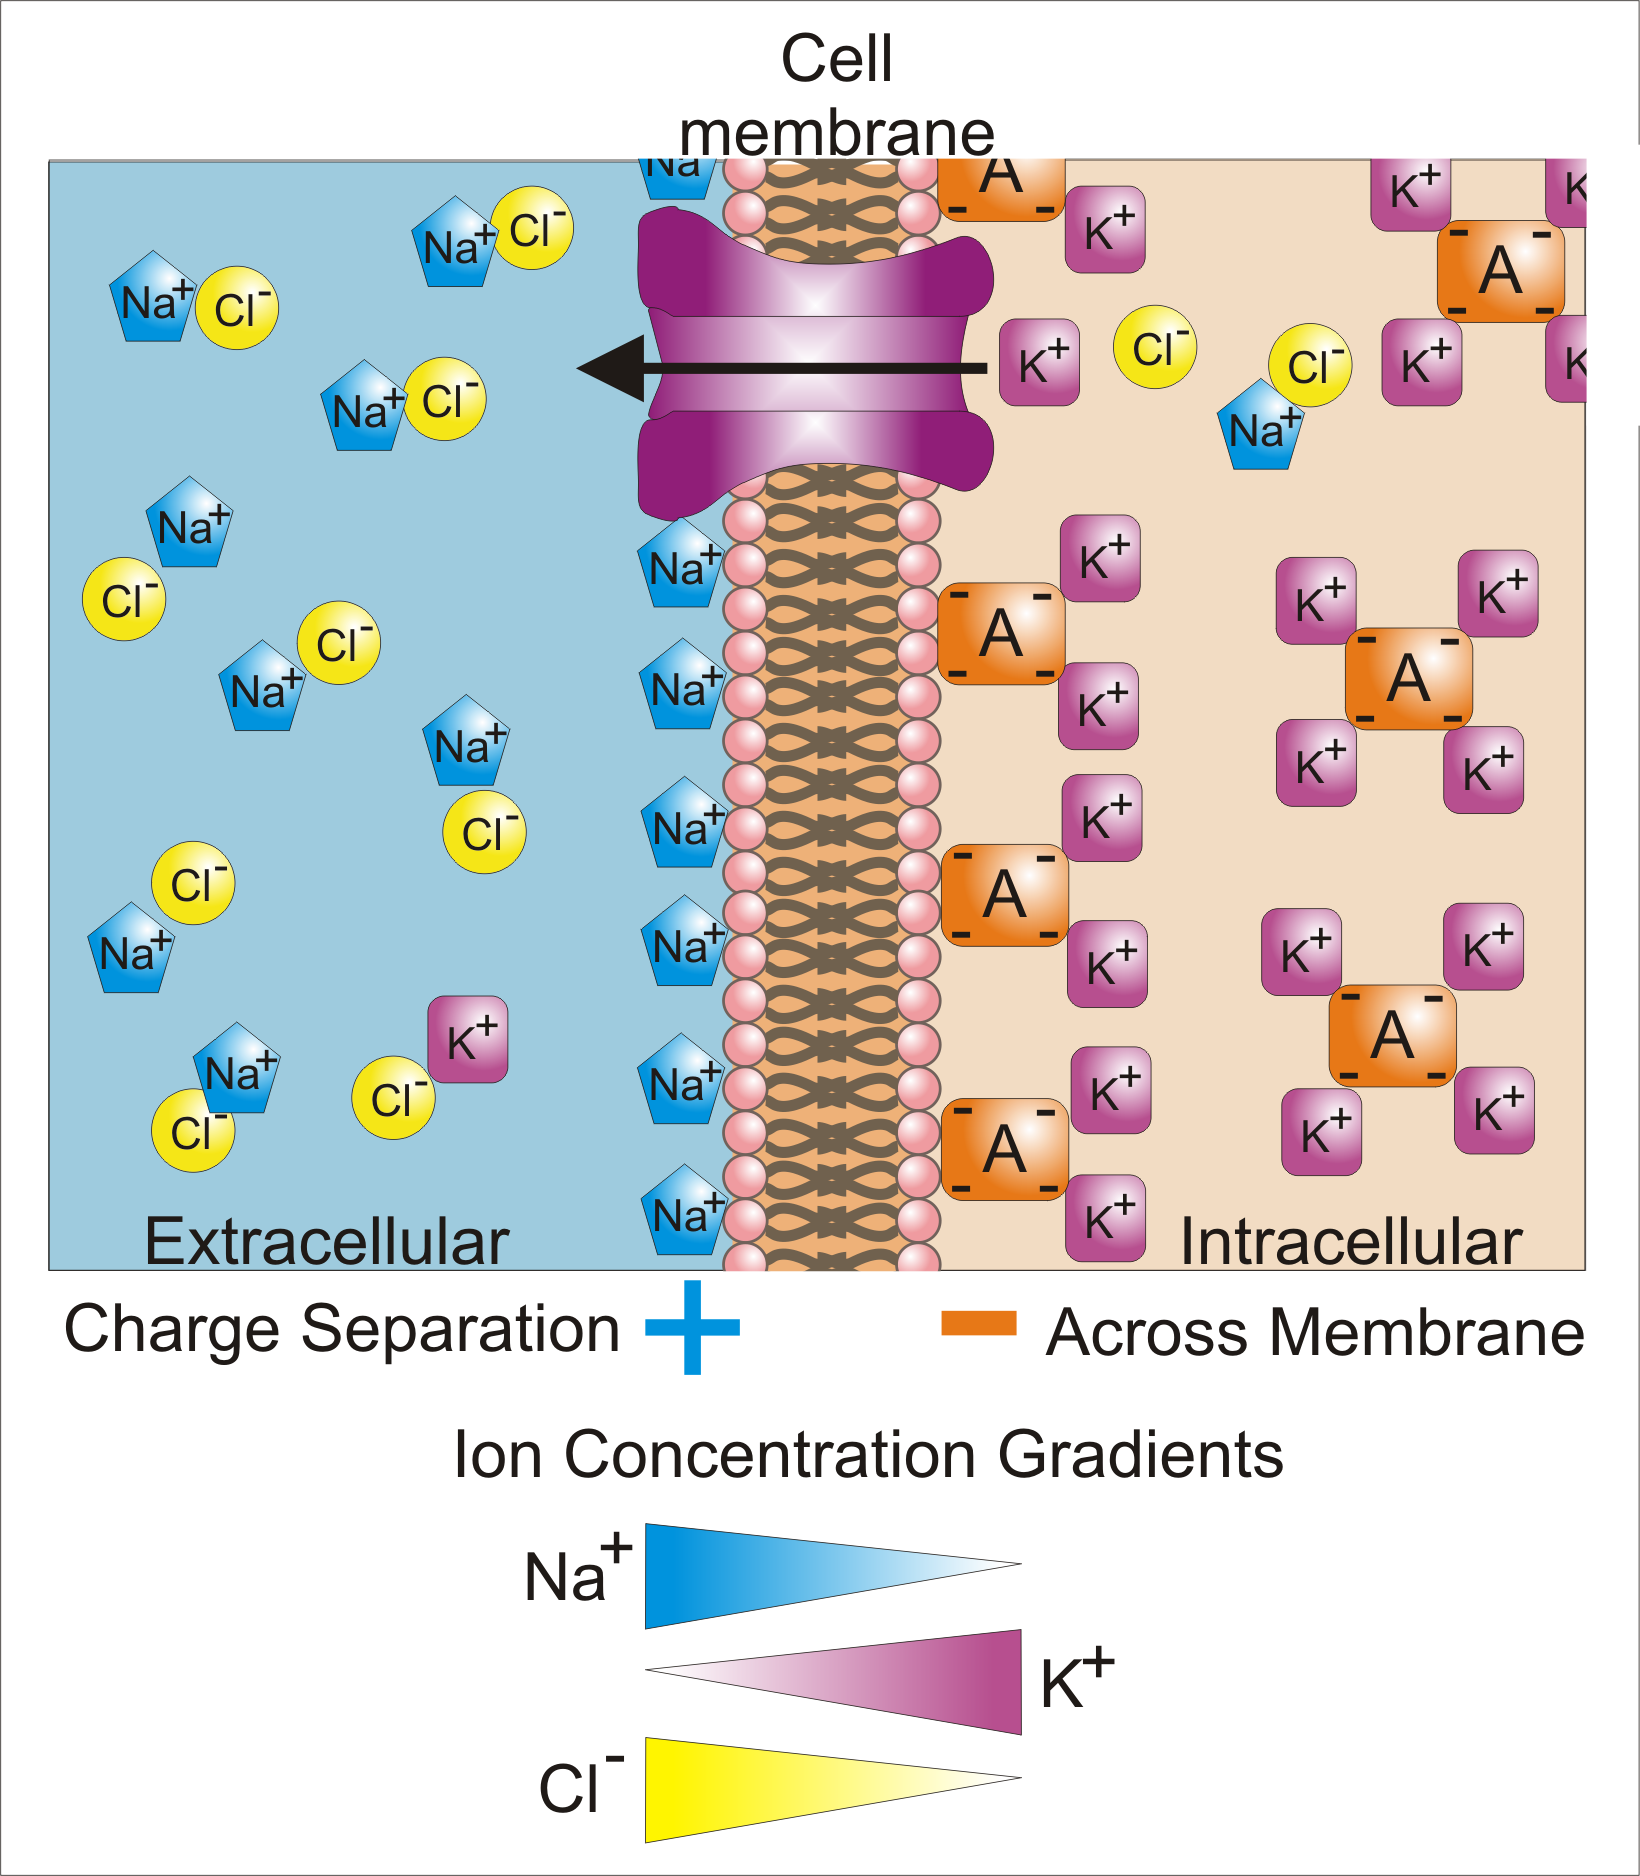
\includegraphics[width=0.40\textwidth]{Figures/neurobiology/membrane_potential}
		\caption{\textbf{Membrane potential:} Basic schema. \\
        \hrulefill \\
        \textit{By Synaptidude - Own work, CC BY-SA 3.0
        \url{https://commons.wikimedia.org/wiki/File:Basis_of_Membrane_Potential2.png} } }
		\label{fig:MembranePotential}
\end{wrapfigure}
These ions cannot simply cross the lipid-bilayer of the cell membrane by themselves.
To do that, they depend on special enzymes embedded into the membrane: ion-channels, ion-pumps and ion-transporters.
Ion-channels can either be permeable \todo{finish this, or don't\dots}

The most important ion-pumps are sodium-potassium pumps, which move potassium into the cell, while expelling sodium.

Sitting in the membrane are multiple kinds of ion-channels that can change the permeability for
specific ions depending on certain factors.
For example, voltage-gated channels open and close depending on the membrane potential,
while ligand-gated channels are controlled by certain chemicals (neurotransmitters) binding to them.



A cell's resting potential primarily depends on the equilibrium state of the potassium ions,
where the influx of potassium ions due to the concentration gradient is equal to the efflux due the voltage gradient.

The membrane potential can leave it's resting state, when processes disturb this balance.
Most commonly, when ligand-gated ion-channels open and let ions enter the cell.
Depending on the type of ion, this can lead to depolarization or hyperpolarization of the membrane potential.
Because depolarization increases the chances of a neuron firing, this process is also described as \textit{excitation},
while polarization, which in turn decreases that chance, is called \textit{inhibition}.
\subsubsection{Action Potential}
When the membrane potential of a Neuron reaches a certain Threshold at the axon hillock, it triggers 
\subsubsection{Synaptic Gap}
\subsubsection{Excitation and Inhibition}
\subsubsection{Post-Synaptic-Potential}
\subsubsection{Axon Hillock}
\subsubsection{Firing Rate}
\subsection{Consciousness on a neural level}\label{subsec:consciousness-on-a-neural-level}

\subsubsection{Influence of GABA-A Sedatives}
% \begin{itemize}
%	\item Recap:
%	\begin{itemize}
%		\item Action potential
%		\item Inhibition/Excitation
%		\item Synaptic Gap
%		\item Post-Synaptic-Potential
%		\item Axon hillock
%		\item Firing rate
%	\end{itemize}
%	\item What do we know about consciousness on a neural level?
%	\begin{itemize}
%		\item How do GABA-A Sedatives (like Propofol) work on a neural level?
%	\end{itemize}
% \end{itemize}